\section{LTI-Systeme}{171}

\begin{tabular}{ll}
	$x(t)$ 				& Eingangssignal 										\\
	$y(t)$ 				& Ausgangssignal 										\\
	$\delta(t)$ 		& Dirac-Stoss 											\\
	$h(t)$ 				& Impulsantwort (Antwort auf Dirac-Stoss) 				\\
	$H(\jimg \omega)$ 	& Frequenzgang 											\\
	$H(s)$ 				& $H(s) = \frac{Y(s)}{X(s)}$ Übertragungsfunktion (UTF)
\end{tabular}


\subsection[Bestimmung des Ausgangssignals]{Bestimmung des Ausgangssignals $\bm{y(t)}$}{173}

Das Ausgangssignal $y(t)$ eines Systems entspricht der \textbf{Faltung} des Eingangssignals $x(t)$ mit der Impulsantwort $h(t)$ des Systems.
$$ \boxed{ y(t) = \int\limits_{-\infty}^{\infty} x(\tau) h(t-\tau) \, \diff \tau = \int\limits_{-\infty}^{\infty} h(\tau) x(t-\tau) \, \diff \tau } $$

Die Faltungsoperation kann auch mit dem \textbf{Stern-Operator} geschrieben werden:
$$ \boxed{ y(t) = x(t) * h(t) = h(t) * x(t) = (x * y)(t) } $$

\vspace{0.2cm}

Im Bildbereich bestimmt man die Fourier-Transformierte der Ausgangsfunktion als:
$$ \boxed{ Y(\jimg \omega) = H(\jimg \omega) \cdot X(\jimg \omega) } \qquad \text{mit } H(\jimg \omega) = \int\limits_{- \infty}^{\infty} h(t) \, e^{- \jimg \omega t} \, \diff t $$


\subsection[Frequenzgang]{Frequenzgang $H\bm{(\jimg \omega)}$}
\label{Frequenzgang}

Der \cor{Frequenzgang $H(\jimg \omega)$} wird häufig als \cbl{Betrag (Amplitudengang)} und \cgn{Phase (Phasengang)} dargestellt:

$$ \boxed{ \cor{H(\jimg \omega)} = \alpha \cdot e^{- \jimg \omega t_0} = \cbl{|H(\jimg \omega)|} \cdot e^{\cgn{\jimg \Theta (\jimg \omega)} } }$$

\vspace{-0.2cm}

\begin{align*}
	\cbl{|H(\jimg \omega)|} 	&= \sqrt{H(\jimg \omega) \cdot \overline{H(\jimg \omega)}} = \sqrt{\mathrm{Re}(H(\jimg \omega))^2 + \mathrm{Im}(H(\jimg \omega))^2}\\
	\cgn{\Theta (\jimg \omega)} &= \arg(H(\jimg \omega)) = 
	\begin{cases}
		\arccos\left(\frac{\RE(H(\jimg \omega))}{|H(\jimg \omega)|}\right)  & \text{für} \; \IM(H(\jimg \omega)) \geq 0 \\
		-\arccos\left(\frac{\RE(H(\jimg \omega))}{|H(\jimg \omega)|}\right) & \text{für} \; \IM(H(\jimg \omega)) < 0
	\end{cases}
\end{align*}

	
\begin{tabular}{ll}
	Amplitudengang: & achsensymmetrisch (gerade) \\
	Phasengang: 	& punktsymmetrisch (ungerade)
\end{tabular}

\vspace{0.2cm}

\textrightarrow\ Ersetzt man im Freqenzgang $\jimg \omega$ durch $s$, so erhält man die Übertragungsfunktion $H(s)$


\subsection{Zusammenhänge zwischen den Grössen}{174-176}

Die Impulsantwort $h(t)$ und der Frequenzgang $H(\jimg \omega)$ sind ein \\
\textbf{Fourier}-Transformationspaar:

\begin{center}
	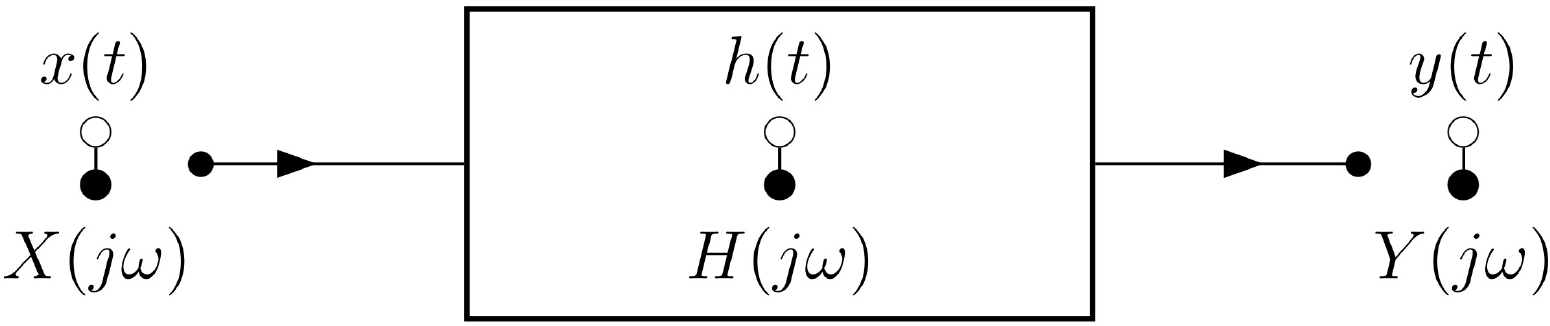
\includegraphics[width=0.6\columnwidth]{images/frequenzgang_impulsantwort.png}
\end{center}

Die Impulsantwort $h(t)$ und die Übertragungsfunktion $H(s)$ sind ein\\
 \textbf{Laplace}-Transformationspaar:
$$ \boxed{ h(t) \, \laplace \, H(s) } $$


Das Ausgangssignal berechnet sich als: 
$$ \boxed{ y(t) = h(t) * x(t) \, \laplace \, Y(s) = H(s) \cdot X(s) } $$


\subsubsection{Zusammenhang Impulsantwort \& Einheitssprungantwort}

\begin{tabular}{ll c c ll}
	$h(t)$ & Impulsantwort 	& 	& $g(t)$ & Einheitssprungantwort 
\end{tabular}

$$ \boxed{ h(t) =  \frac{\diff g(t)}{\diff t}  \quad \Leftrightarrow \quad g(t) = \int\limits_{-\infty}^t  h(\tau) \, \diff \tau }  $$
$$ \boxed{ H(s) = s \cdot G(s) \quad \Leftrightarrow \quad G(s) = \frac{1}{s} H(s) }  $$


\subsubsection{Zusammenhang Impulsantwort \& Kausalität LTI-System}

\fbox{\parbox{0.9\columnwidth}{
Damit ein LTI-System kausal ist, muss dessen Impulsantwort $h(t)$ für alle $t < 0$ gleich Null sein. 
} }


\subsection{Zusammenschalten von LTI-Systemen}

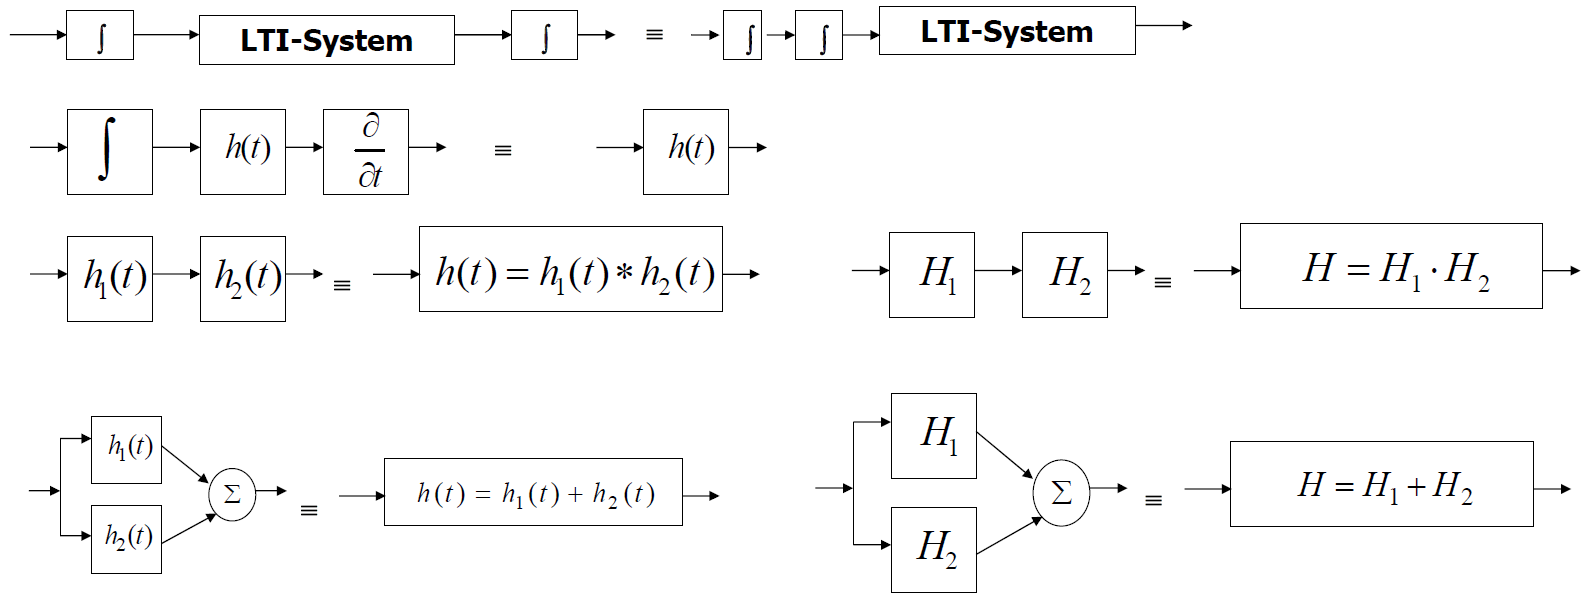
\includegraphics[width=\columnwidth]{images/zusammenschalten_von_LTI_systemen.png}


\subsection{Stabilität von LTI-Systemen}{177-181}

Bei den Betrachtungen von LTI-Systemen nehmen wir jeweils an, dass die Systeme \textbf{kausal} sind!


\subsubsection{BIBO-Stabilität}{177}

BIBO: \textbf{B}ounded \textbf{I}nput \textbf{B}ounded \textbf{O}utput

\vspace{0.2cm}

Ein LTI-System ist BIBO-stabil, wenn die \textbf{Impulsantwort absolut integrierbar} ist:

$$ \boxed{ \int\limits_{-\infty}^{\infty} |h(t)| \, \diff t < \infty } $$

\textrightarrow\ Für ein beschränktes Eingangssignal $x(t)$ ist auch das Ausgangssignal $y(t)$ beschränkt.


\subsubsection{Asymptotische Stabilität}{178}

Ein LTI-System ist asymptotisch stabil, wenn seine \textbf{Impulsantwort asymptotisch gegen Null} abklingt.

$$ \boxed{ \lim\limits_{t \to \infty} h(t) = 0 } $$

Alle kausalen LTI-Systeme mit \textbf{Polen nur in der linken $\bm{s}$-Halbebene} sind asymptotisch stabil! ($\sigma < 0$) \\
\textrightarrow\ Siehe Konvergenzhalbebene Abschnitt \ref{Konvergenzhalbebene}


\subsubsection{Instabilität}{178}

Ein LTI-System ist instabil, wenn: (ODER-Verknüpfung)

\vspace{0.1cm}

\begin{itemize}
	\item mindestens ein Pol der UTF in der \textbf{rechten $\bm{s}$-Halbebene} liegt ($\sigma > 0$) 
	\item mindestens ein \textbf{mehrfacher Pol auf der $\bm{\jimg \omega}$-Achse} der
		$s$-Ebene liegt (Pole müssen am gleichen Ort sein!) 
\end{itemize}


\subsubsection{Grenzstabilität}{178}

Ein LTI-System ist grenzstabil (quasistabil), wenn: (UND-Verknüpfung)

\vspace{0.1cm}

\begin{itemize}
	\item \textbf{kein} Pol in der rechten $s$-Halbebene liegt  ($\sigma < 0$)
	\item kein mehrfacher Pol auf der $\jimg \omega$-Achse der $s$-Ebene liegt
	\item auf der $\jimg \omega$-Achse mindestens ein \textbf{einfacher Pol} ist
\end{itemize}

\vspace{0.2cm}

\begin{minipage}[c]{0.6\columnwidth}
	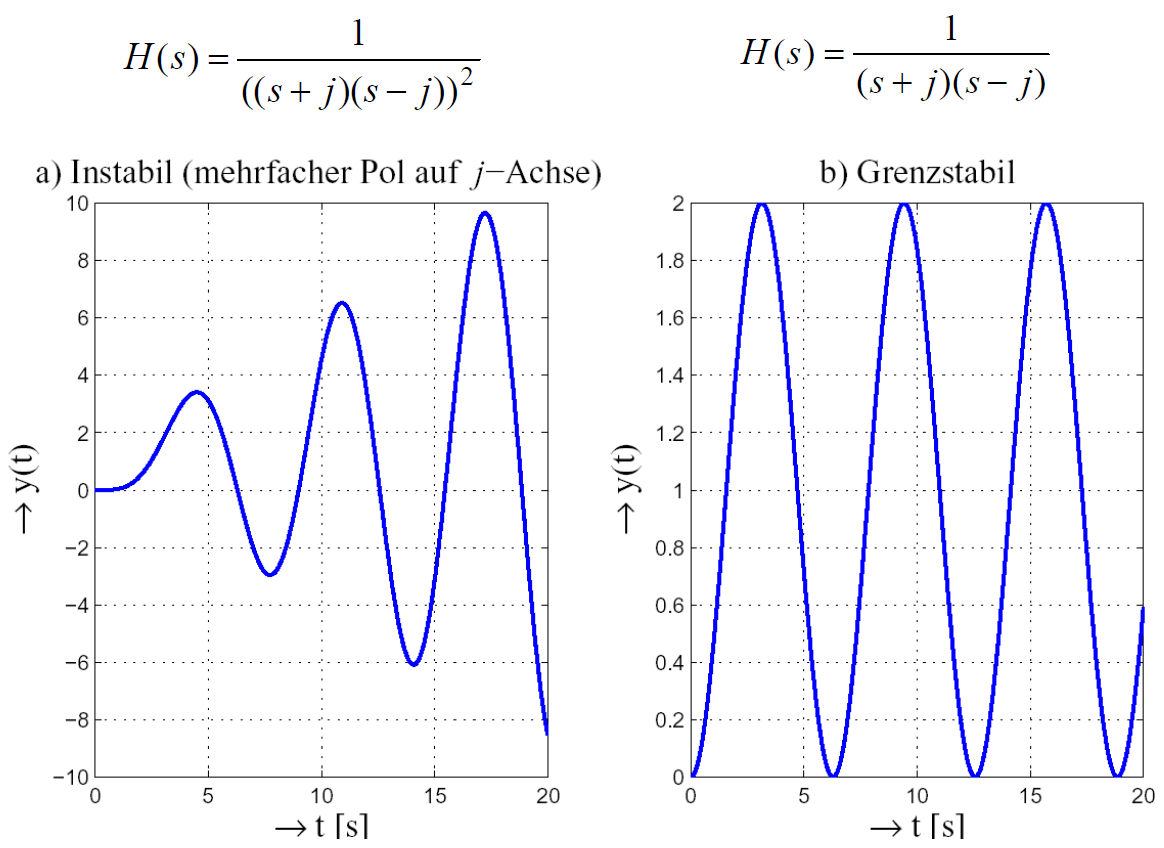
\includegraphics[width=\columnwidth]{images/grenzstabilitaet.png}
\end{minipage}
\hfill
\begin{minipage}[c]{0.38\columnwidth}
	\raggedright
	Ein System ist grenzstabil, wenn die Amplitude eines Signals 'erhalten' bleibt 
\end{minipage}


\subsubsection{Algebraische Stabilitätskriterien}{179-181}

\vspace{-0.2cm}
$$ P(s) = X(s) = a_n s^n + a_{n-1} s^{n-1} + ... + a_1 s + a_0 = a_n(s-p_1) \cdot ... \cdot (s-p_n) $$

Das Stabilitätskriterium betrachtet den \textbf{Nennen} $\boldsymbol{D(s)}$ der Übertragungsfunktion 
$$ H(s) = \frac{Y(s)}{X(s)} = \frac{N(s)}{D(s)}$$

\begin{itemize}
	\item Wenn der \textbf{Nenner} $\boldsymbol{D(s)}$ ein \textbf{Hurwitz-Polynom} ist, so ist das System \textbf{asymptotisch stabil.}
	\item Ein \textbf{modifiziertes Hurwitz-Polynom} ergibt ein \textbf{grenzstabiles System} \\
		\textrightarrow\ Polynom braucht \textbf{einfache Nullstellen} auf $\jimg \omega$-Achse
\end{itemize}

\vspace{0.3cm}

\myul{\textbf{Hurwitz-Kriterium}}

\vspace{0.1cm}

Ein Polynom $P(s)$ ist nur dann ein Hurwitz-Polynom wenn folgende \textbf{beiden} Bedingungen erfüllt sind: 

\vspace{0.1cm}

\begin{enumerate}
	\item Die Vorzeichen aller Koeffizienten $a_i$ von $P(s)$ sind \textbf{identisch} (und alle Koeffizienten $a_i$ sind vorhanden)
	\item Alle Hurwitz-Determinanten $D_1$ bis $D_n$ sind grösser als Null
\end{enumerate}

\vspace{0.3cm}

\myul{\textbf{Hurwitz-Determinanten}}

\begin{minipage}[c]{0.23\columnwidth}
	$$ D_1 = a_{n-1} > 0 $$
\end{minipage}
\hfill
\begin{minipage}[c]{0.27\columnwidth}
	$$ D_2 = 
	\begin{vmatrix}
		a_{n-1} & a_n \\
		a_{n-3} & a_{n-2} 
	\end{vmatrix}  > 0 $$
\end{minipage}
\hfill
\begin{minipage}[c]{0.45\columnwidth}
	$$ D_3 = \begin{vmatrix}
		a_{n-1} & a_n 		& 0			\\	
		a_{n-3} & a_{n-2} 	& a_{n-1} 	\\
		a_{n-5} & a_{n-4} 	& a_{n-3} 
	\end{vmatrix}  > 0 $$
\end{minipage}


\begin{minipage}[c]{0.6\columnwidth}
	$$ D_{n-1} = \begin{vmatrix}
		a_{n-1} & a_n 		& 0 		& 0 		& \cdots 	& 0 	\\
		a_{n-3} & a_{n-2} 	& a_{n-1} 	& a_n 		& 0 		& 0 	\\
		a_{n-5} & a_{n-4} 	& a_{n-3} 	& a_{n-2}	& \cdots 	& 0 	\\
		\vdots 	& \vdots  	& \vdots  	& \vdots  	& \ddots 	& 0 	\\
		0 		& 0 		& 0 		& \cdots 	& 0 		& a_1 
	\end{vmatrix}  > 0 $$
\end{minipage}
\hfill
\begin{minipage}[c]{0.38\columnwidth}
	$$ D_n = a_0 \, D_{n-1} > 0  $$
\end{minipage}


\subsection[Phasenlaufzeit]{Phasenlaufzeit $\tau_P(\omega)$}{183}

Die Phasenlaufzeit ist nur für \textbf{reine Sinus-Schwingungen} exakt bestimmbar! \\
Das System ist beschrieben durch:
$$ x(t) = A \cdot \sin(\omega_0 t + \gamma)$$
$$ H( \jimg \omega) = \alpha \cdot e^{- \jimg \omega t_0} \, \laplace \, h(t) = \alpha \cdot \delta(t - t_0) $$


Das Ausgangssignal $y(t) = x(t) * h(t)$ ist gegenüber dem Eingangssignal $x(t)$ mit $\alpha$ gewichtet und um die Zeit $t_0$ verzögert. \\
\textrightarrow\ \textbf{Diese Verzögerung wird Phasenlaufzeit genannt}

$$ \boxed{ \tau_P(\omega) = \frac{- \theta(\omega)}{\omega} } $$

$ \theta(\omega)$ entspricht dem Phasengang des Systems \textrightarrow\ Siehe Abschnitt \ref{Frequenzgang}


\example{Phasenlaufzeit}

\begin{center}
	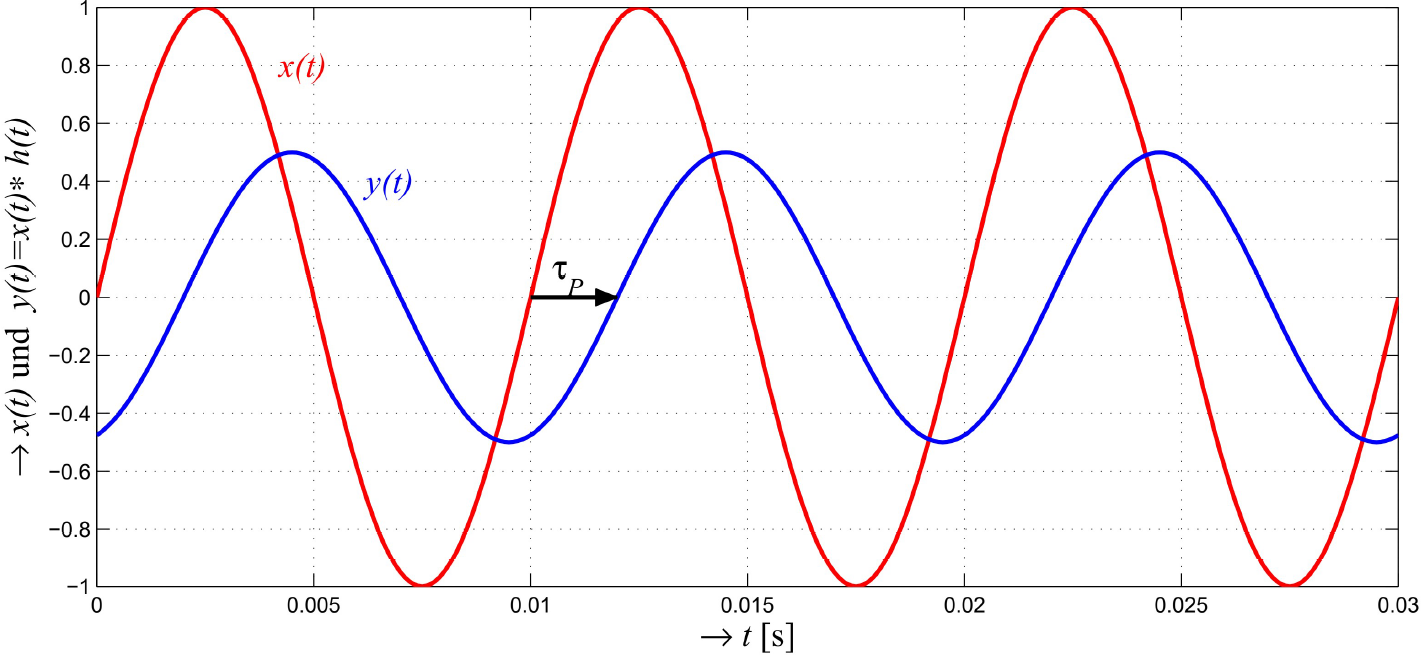
\includegraphics[width=0.8\columnwidth]{images/phasenlaufzeit.png}
\end{center}


\subsubsection{Negative Phasenlaufzeit}

Eine negative Phasenlaufzeit bedeutet \textbf{nicht}, dass ein System \textbf{akausal} ist!


\subsection[Gruppenlaufzeit]{Gruppenlaufzeit $\tau_G(\omega)$}

Definiert für Signale mit \textbf{mehreren Frequenzanteilen}

\vspace{0.2cm}

Bei amplitudenmodulierten Signalen bestimmt die Gruppenlaufzeit $\tau_G(\omega)$ die \textbf{Verzögerung der Hüllkurve} der AM.

$$ \boxed{ \tau_G(\omega) = \frac{- \diff \theta(\omega)}{\diff \omega} } $$

$ \theta(\omega)$ entspricht dem Phasengang des Systems \textrightarrow\ Siehe Abschnitt \ref{Frequenzgang}

\vspace{0.2cm}

Die Gruppenlaufzeit kann nur dann als \textbf{Laufzeit des Signals} interpretiert werden, wenn im Frequenzbereich des Signales die Gruppenlaufzeit und auch die Dämpfung ungefähr konstant sind.


\subsubsection{Negative Gruppenlaufzeit}

Bei \textbf{Vierpolen} mit \textbf{konzentrierten Elementen} ist in bestimmten Frequenzbereichen eine \textbf{negative Gruppenlaufzeit} 
möglich, insbesondere in Frequenzbereichen wo die Dämpfung stark ändert. (z.B. Nullstellen der UTF)

\vspace{0.2cm}

Bei negativer Gruppenlaufzeit erscheint die Wirkung \textbf{nicht} vor der Ursache! \\
\textrightarrow\ Das System ist \textbf{nicht} akausal! \\
Das Maximum der Hüllkurve kann am Ausgang kann aber \textbf{früher} als am Eingang auftreten.



\subsection{Phasenlaufzeit / Gruppenlaufzeit identisch}{186}

Die \textbf{Signalverzögernug, Phasenlaufzeit} $\bm{\tau_P(\omega)}$ und \textbf{Gruppenlaufzeit} $ \bm{\tau_G(\omega)}$ sind identisch, 
wenn
$$ \boxed{ \theta(\omega) = - \omega \cdot t_0  } $$

und der \textbf{Amplitudengang ebenfalls konstant} ist, d.h., $H(\jimg \omega) = \alpha \cdot e^{-\jimg \omega t_0}$ 

\vspace{0.2cm}

Die Signalverzögerung beträgt für \textbf{alle Frequenzen} $t_0 (= \tau_P = \tau_G) $ 




\subsection{Verzerrungen}{187-188}

Stimmt der zeitliche Verlauf einer Schwingung auf der Empfängerseite nicht mehr mit der Senderseite überein, arbeitet das 
Übertragungssystem \textbf{nicht verzerrungsfrei}.


\subsubsection{Lineare Verzerrung}

Eine \textbf{Dämpfung} eines Signals (z.B. durch einen Tiefpassfilter) entspricht einer \textbf{linearen Verzerrung}.


\subsubsection{Nichtlineare Verzerrung}

Nichtlineare Verzerrungen werden durch \textbf{Übersteuerung} des Systems \textbf{(Kanal)} oder dessen \textbf{nichtlineare Kennlinie} 
hervorgerufen.

\vspace{0.1cm}

Durch nichtlineare Verzerrungen treten \textbf{neue}, im Ursprungssignal nicht enthaltene \textbf{Schwingungen} auf.

\vspace{0.1cm}

Ein \textbf{Mass} für nichtlineare Verzerrungen ist der \textbf{Klirrfaktor}.


\subsection{Klirrfaktor}{186}

Verhältnis des \textbf{Effektivwerts} der \textbf{neu} am Ausgang eines Systems entstandenen \textbf{Harmonischen} zum Effektivwert des 
gesamten Signals.

\vspace{0.2cm}

\begin{minipage}[c]{0.55\columnwidth}
	$$ \boxed{ k = \sqrt{\frac{U_2^2 + U_3^2 + ...+ U_n^2}{U_1^2 + U_2^2 + ...+ U_n^2}}} $$
\end{minipage}
\hfill
\begin{minipage}[c]{0.4\columnwidth}
	Es gilt: $1 > k \geq 0$
\end{minipage}

\vspace{0.2cm}

$U_1$ entspricht der Grundharmonischen!


\subsubsection{Klirrdämpfungsmass}

\vspace{-0.2cm}
$$ \boxed{ a_k = 20 \cdot \log_{10} \Big( \frac{1}{k}  \Big)  } $$


\subsubsection{Total Harmonic Disortion (THD)}

Wird vor allem im englisch-sprachigen Raum verwendet

\vspace{0.2cm}

\begin{minipage}[c]{0.55\columnwidth}
	$$ \boxed{  \text{THD} = \sqrt{\frac{U_2^2 + U_3^2 + ...+ U_n^2}{U_1^2} } } $$
\end{minipage}
\hfill
\begin{minipage}[c]{0.4\columnwidth}
	Es gilt: $\infty > \text{THD} \geq 0$
\end{minipage}

\vspace{0.2cm}

$U_1$ entspricht der Grundharmonischen! 

\vspace{0.2cm}
\begin{itemize}
	\item Für geringe Verzerrungen gilt: $\text{THD} \approx k$
	\item Im Allgemeinen gilt: $\text{THD} > k$
\end{itemize}

